\documentclass[14pt, a4paper]{report}
\usepackage{mathtext}
\usepackage[T2A]{fontenc}
\usepackage[utf8]{inputenc}
\usepackage[russian]{babel}
\usepackage{multirow}
\usepackage{slashbox}
\usepackage{makecell}
\usepackage{graphicx}
\usepackage{physics}
\usepackage{amstext}
\usepackage{caption}
\usepackage{subcaption}
\usepackage{cmap}
\usepackage{float}
\usepackage{indentfirst}
\usepackage{romannum}
\usepackage{wasysym}

\usepackage[a4paper,
            		left=1in,
            		right=1in,
           		 top=1in,
            		bottom=1in,
            		footskip=.25in]{geometry}

\renewcommand{\thesection}{\arabic{section}.}
\renewcommand{\thesubsection}{\arabic{section}.\arabic{subsection}.}

\title{\textbf{Отчет о выполнении лабораторной работы 5.5. "Компьютерная сцинтилляционная $\gamma$ - спектрометрия"}}
\author{Калашников Михаил, Б03-202}
\date{}

\begin{document}
\maketitle

\pagenumbering{arabic}

\section{Теоретические сведения}

Основными процессами взаимодействия гамма-излучения с веществом являются, как было выше указано, фотоэффект, эффект Комптона и образование электрон-позитронных пар. Каждый из этих процессов вносит свой вклад в образование наблюдаемого спектра.

\textbf{Фотоэффект} -- процесс взаимодействия гамма-кванта с электроном, связанным с атомом, при котором электрону передается вся энергия гамма-кванта. При этом электрону сообщается кинетическая энергия $Т_e = Е_\gamma-I_i$, где $Е_\gamma$ -- энергия гамма-кванта, $I_i$ -- потенциал ионизации i-той оболочки атома. Фотоэффект особенно существенен для тяжелых веществ, где он идет с заметной вероятностью даже при высоких энергиях гамма-квантов. В легких веществах фотоэффект становится заметен лишь при относительно небольших энергиях гамма-квантов.

\textbf{Эффект Комптона} -- упругое рассеяние фотона на свободном электроне, сопровождающееся изменением длины волны фотона (реально этот процесс происходит на слабо связанных с атомом внешних электронах). Максимальная энергия образующихся комптоновских электронов соответствует рассеянию гамма-квантов на $180^\circ$ и равна

\[E_{max}=\frac{\hbar\omega}{1+\frac{mc^2}{2\hbar\omega}}\text{.}\]

\textbf{Процесс образования электрон-позитронных пар.} При достаточно высокой энергии гамма-кванта наряду с фотоэффектом и эффектом Комптона может происходить третий вид взаимодействия гамма-квантов с веществом -- образование электрон-позитронных пар. Процесс образования пар не может происходить в пустоте, так как в этом случае не выполняются совместно законы сохранения энергии и импульса. В присутствии ядра или электрона процесс образования пары гамма-квантом возможен, так как можно распределить энергию и импульс гамма-кванта между тремя частицами без противоречия с законами сохранения. При этом если процесс образования пары идет в кулоновском поле ядра, то энергия образующегося ядра отдачи оказывается весьма малой, так что пороговая энергия гамма-кванта $E_{пор}$, необходимая для образования пары, практически совпадает с удвоенной энергией покоя электрона $E_{пор}\approx 2mc^2 =1.022\ МэВ$.

\section{Экспериментальная установка}

\begin{figure}[H]
\centering
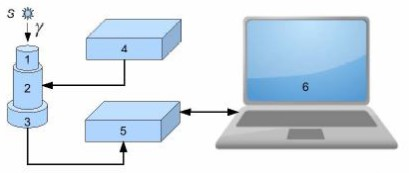
\includegraphics[scale=1]{../images/555-1}
\caption{Принципиальная блок-схема спектрометра. (1 -- сцинтиллятор, 2 -- ФЭУ, 3 -- предусилитель импульсов, 4 -- высоковольтный блок питания для ФЭУ, 5 -- блок преобразования аналоговых импульсов с ФЭУ в цифровой код (АЦП), 6 -- компьютер для сбора данных, их обработки и хранения).}
\end{figure}

ФЭУ со сцинтиллятором и блоком питания установлены на отдельной подставке. В нашей работе на разных установках (стендах) в качестве сцинтиллятора используются кристаллы NaI(Tl) с размерами $\diameter\ 45\times50\ мм$ и $\diameter\ 20\times25\ мм$.

\section{Проведение эксперимента}

\section{Обработка результатов}

\section{Выводы}

\end{document}